\chapter{Game Theory}

\begin{lemma}
	For every game $G$, there exists at least one individually rational strategy profile.
	In other words, $\mathcal{S}_1(G) \ne \emptyset$.
\end{lemma}

\begin{proof}
	For every player $i \in P$ we denote $m_i = \text{arg} \max_{t_i \in S_i} \min_{\vect_{-i} \in S_{-i}} u_i(t_i, \vect_{-i}) \in S_i$ the strategy that lower-bounds utility of player $i$.
	We claim that the strategy profile $\mm = (m_1, \dots, m_n) \in S$ is individually rational.
	If $\mm$ was not individually rational, there would have to be some player $j \in P$ and a strategy $s_j^* \in S_j$ that would ensure a better worst-case payoff: $\min_{\vecs_{-j} \in S_{-j}}u_j(s_j^*, \vecs_{-j}) > u_j(\mm)$ which would contradict the choice of $m_j$.
\end{proof}

\section{General games without ties}

\begin{observation}
	\label{th:pte-subset-ir}
	If a game $G = (P, S, \uu)$ has a PTE $\vecs \in S$, then $\vecs$ is individually rational.
	However, not every individually rational profile is a PTE.
	In other words, if we think of PTE and IR as sets of strategy profiles in any given game, we have PTE $\subsetneq$ IR.
\end{observation}

\begin{definition}[Perfectly transparent best response]
	For a game $G = (P, S, \uu)$ we say a strategy $s_i^* \in S_i$ is a perfectly transparent best response to a strategy profile $\vecs_{-i}$ of the opponent players if it is the Nashian best response to $\vecs_{-i}$ across all profiles that survive the maximum number of preemption rounds before all possible profiles are eliminated.
	Formally, there is some $k \in \N$ such that $(s_i^*, \vecs_{-i}) \in \mathcal{S}_k$, and $(s_i, \vecs_{-i}) \notin \mathcal{S}_{k+1} \forall s_i \in S_i$, and
	\[
		u_i(s_i^*, \vecs_{-i}) \ge u_i(s_i', \vecs_{-i})\ \forall (s_i', \vecs_{-i}) \in \mathcal{S}_k.
	\]
\end{definition}

\begin{definition}[Perfectly transparent best response equilibrium]
	We say a strategy profile $\vecs = (s_1, \dots, s_n) \in S$ is a perfectly transparent best response equilibrium (PTBRE) if $s_i$ is a perfectly transparent best response to $\vecs_{-i}$ for all players $i \in P$.
\end{definition}

\begin{observation}
	\label{th:tbre-subset-pte}
	If a strategy profile is a PTE, then it must be a PTBRE; we have PTE $\subset$ PTBRE.
\end{observation}

\begin{remark}
	The other inclusion does not hold: PTBRE $\not\subseteq$ PTE.
	A counterexample is displayed in \autoref{tab:pte-ne-ptbre}.
	Thus, we have PTE $\subsetneq$ PTBRE.
\end{remark}

\begin{table}
	\caption{
		An example game showing that PTE $\ne$ PTBRE.
		Profiles eliminated in the first round are highlighted in \colorbox{gray!70}{dark-grey}.
		Profiles eliminated in the second round are highlighted in \colorbox{gray!20}{light-grey}.
		We see that the profiles (B, E) and (C, D) are is not PTE but they are PTBRE.
	}
	\label{tab:pte-ne-ptbre}
	\centering
	\begin{tabular}{|c|c|c|c|}
		\hline
			& D		& E	   & F	  \\
		\hline
		A 		&\cellcolor{gray!70} 6, 2 &\cellcolor{gray!20} 3, 5 &\cellcolor{gray!70} 0, 0 \\
		\hline
		B		&\cellcolor{gray!70} 7, 1 &\cellcolor{gray!20} 8, 3 &\cellcolor{gray!70} 1, 6 \\
		\hline
		C		&\cellcolor{gray!20} 5, 8 &\cellcolor{gray!20} 2, 7 &\cellcolor{gray!20} 4, 4 \\
		\hline
	\end{tabular}
\end{table}

\begin{table}
	\caption{
		An example game for which a PTBRE does not exist.
		Profiles eliminated in the first round are highlighted in \colorbox{gray!70}{dark-grey}.
		Profiles eliminated in the second round are highlighted in \colorbox{gray!20}{light-grey}.
		The perfectly transparent best responses of the row player to D, E, F are B, A, B, respectively.
		The perfectly transparent best responses of the column player to A, B, C are F, E, F, respectively.
	}
	\label{tab:no-ptbre}
	\centering
	\begin{tabular}{|c|c|c|c|}
		\hline
			& D		& E	   & F	  \\
		\hline
		A 		&\cellcolor{gray!70} 1, 1 &\cellcolor{gray!20} 8, 4 &\cellcolor{gray!20} 5, 5 \\
		\hline
		B		&\cellcolor{gray!20} 3, 7 &\cellcolor{gray!20} 4, 8 &\cellcolor{gray!20} 6, 3 \\
		\hline
		C		&\cellcolor{gray!70} 7, 2 &\cellcolor{gray!70} 0, 0 &\cellcolor{gray!70} 2, 6 \\
		\hline
	\end{tabular}
\end{table}

\begin{lemma}
	For any game $G = (P, S, \uu)$, if a strategy profile $\vecs \in S$ is a PTBRE, then it is individually rational.
\end{lemma}

\begin{proof}
	Let us suppose that there is a game $G = (P, S, \uu)$ and a strategy profile $\vecs = (s_1, \dots, s_n) \in S$ such that $\vecs$ is a PTBRE but not individually rational.
	This is equivalent to $s_i$ being a perfectly transparent best response to $\vecs_{-i}$ for all $i \in P$, and $\vecs \notin \mathcal{S}_1$.
	Note that we must also have $(s_i', \vecs_{-i}) \notin \mathcal{S}_1\ \forall s_i' \in S_i,\ \forall i \in P$ because otherwise $s_i$ would not be a perfectly transparent best response to $\vecs_{-i}$ for some player $i$.
	This means the perfetcly transparent best response of every player $i \in P$ to $\vecs_{-i}$ is simply a Nashian best response (since all considered strategy profiles are eliminated in the same preemption round).
	Thus, $\vecs$ is a Nash equilibrium, which is always individually rational.
\end{proof}

\begin{definition}[Perfectly transparent $i$-best profile]
	For a game $G = (P, S, \uu)$ and player $i \in P$ we say a strategy profile $\vecs = (s_1, \dots, s_n) \in S$ is a perfectly transparent $i$-best profile if
	$s_i$ is a perfectly transparent best response to $\vecs_{-i}$ and $u_i(\vecs) \ge u_i(b(\vecs'_{-i}), \vecs'_{-i})$ for all opponent profiles $\vecs'_{-i}$ where $b(\vecs'_{-i})$ is the perfectly transparent best response to $\vecs'_{-i}$.
\end{definition}

\begin{definition}[Perfectly transparent best profile equilibrium]
	We say a strategy profile $\vecs \in S$ is a perfectly transparent best profile equilibrium (PTBPE) if $\vecs$ is a perfectly transparent $i$-best profile for all $i \in P$.
\end{definition}

\begin{lemma}
	If a game $G = (P, S, \uu)$ has a PTBPE $\vecs \in S$, then $\vecs$ is also a PTE, i.e., we have the inclusion PTBPE $\subset$ PTE.
\end{lemma}

\begin{proof}
	For the sake of deriving a contradiction, suppose that there is a game $G = (P, S, \uu)$ with a strategy profile $\vecs = (s_1, \dots, s_n) \in S$ such that $\vecs$ is a PTBPE but not a PTE and let $k$ be the last preemption round in which $\vecs$ is not eliminated (i.e., $\vecs \in \mathcal{S}_k$ but $\vecs \notin \mathcal{S}_{k+1}$).
	Because $\vecs$ is eliminated in the $(k+1)$\textsuperscript{st} round, there must be some player $i \in P$ with a strategy $s_i^* \ne s_i$ which causes the elimination:
	\[
		\forall \vecs_{-i}' \in S_{-i}: (s_i^*, \vecs_{-i}') \in \mathcal{S}_k \implies u_i(s_i^*, \vecs_{-i}') > u_i(\vecs).
	\]
	Let $\vecs_{-i}^* \in S_{-i}$ such that $(s_i^*, \vecs_{-i}^*)\in \mathcal{S}_k$ (there must be at least one to cause $\vecs \notin \mathcal{S}_{k+1}$).
	We have $u_i(s_i^*, \vecs_{-i}^*) > u_i(\vecs)$ which means $s_i$ is not a perfectly transparent best response of player $i$ to $\vecs_{-i}$, so $\vecs$ is not a perfectly transparent $i$-best profile, contradicting $\vecs$ being a PTBPE.
\end{proof}

\begin{corollary}
	Since PTBPE $\subset$ PTE, we have
	\begin{itemize}
		\item PTBPE $\subsetneq$ IR (by \autoref{th:pte-subset-ir}), and
		\item PTBPE $\subsetneq$ PTBRE (by \autoref{th:tbre-subset-pte}).
	\end{itemize}
\end{corollary}

\begin{remark}
	The other inclusion does not hold: PTE $\not\subseteq$ PTBPE.
	A counterexample is displayed in \autoref{tab:pte-ne-ptbpe}.
\end{remark}

\begin{table}
	\caption{
		An example game showing that PTE $\ne$ PTBPE.
		Profiles eliminated in the first round are highlighted in \colorbox{gray!70}{dark-grey}.
		Profiles eliminated in the second round are highlighted in \colorbox{gray!20}{light-grey}.
		The white profile (A, A) is a PTE.
		We see that profile (B, F) is a perfectly transparent row-best profile and (C, E) is a perfectly transparent column-best profile, so there is no PTBPE.
	}
	\label{tab:pte-ne-ptbpe}
	\centering
	\begin{tabular}{|c|c|c|c|}
		\hline
			& D		& E	   & F	  \\
		\hline
		A 		&\cellcolor{gray!00} 7, 5 &\cellcolor{gray!70} 2, 2 &\cellcolor{gray!70} 1, 0 \\
		\hline
		B		&\cellcolor{gray!70} 4, 1 &\cellcolor{gray!20} 3, 3 &\cellcolor{gray!20} 8, 4 \\
		\hline
		C		&\cellcolor{gray!70} 0, 7 &\cellcolor{gray!20} 6, 6 &\cellcolor{gray!20} 5, 8 \\
		\hline
	\end{tabular}
\end{table}

\begin{table}
	\caption{
		An example game for which a PTBPE is not minimax rationalizable.
		In the first copy of the table, preemptively eliminated strategies (used for computing the PTBPE) are highlighted.
		In the second copy, minimax dominated strategies (i.e., those that are not minimax rationalizable) are higlighted.
		Profiles eliminated in different rounds are highlighted in different shades: \colorbox{gray!80}{first round}, \colorbox{gray!60}{second round}, \colorbox{gray!40}{third round}, \colorbox{gray!20}{fourth round}.
		Strategy profile (B, F) is a PTBPE, and the only minimax rationalizable profile is (C, F).
	}
	\label{tab:ptbpe-ne-minimax}
	\centering
	\begin{tabular}{|c|c|c|c|}
		\hline
			& D		& E	   & F	  \\
		\hline
		A 		&\cellcolor{gray!80} 1, 1 &\cellcolor{gray!80} 2, 2 &\cellcolor{gray!80} 3, 4 \\
		\hline
		B		&\cellcolor{gray!80} 4, 5 &\cellcolor{gray!40} 6, 8 &\cellcolor{gray!00} 7, 9 \\
		\hline
		C		&\cellcolor{gray!60} 5, 6 &\cellcolor{gray!80} 8, 3 &\cellcolor{gray!60} 9, 7 \\
		\hline
	\end{tabular}
	\hspace{1em}
	\begin{tabular}{|c|c|c|c|}
		\hline
			& D		& E	   & F	  \\
		\hline
		A 		&\cellcolor{gray!80} 1, 1 &\cellcolor{gray!80} 2, 2 &\cellcolor{gray!80} 3, 4 \\
		\hline
		B		&\cellcolor{gray!60} 4, 5 &\cellcolor{gray!40} 6, 8 &\cellcolor{gray!40} 7, 9 \\
		\hline
		C		&\cellcolor{gray!60} 5, 6 &\cellcolor{gray!20} 8, 3 &\cellcolor{gray!00} 9, 7 \\
		\hline
	\end{tabular}
\end{table}

\begin{figure}
	\caption{A venn diagram depicting the inclusion of different equilibria.}
	\centering

	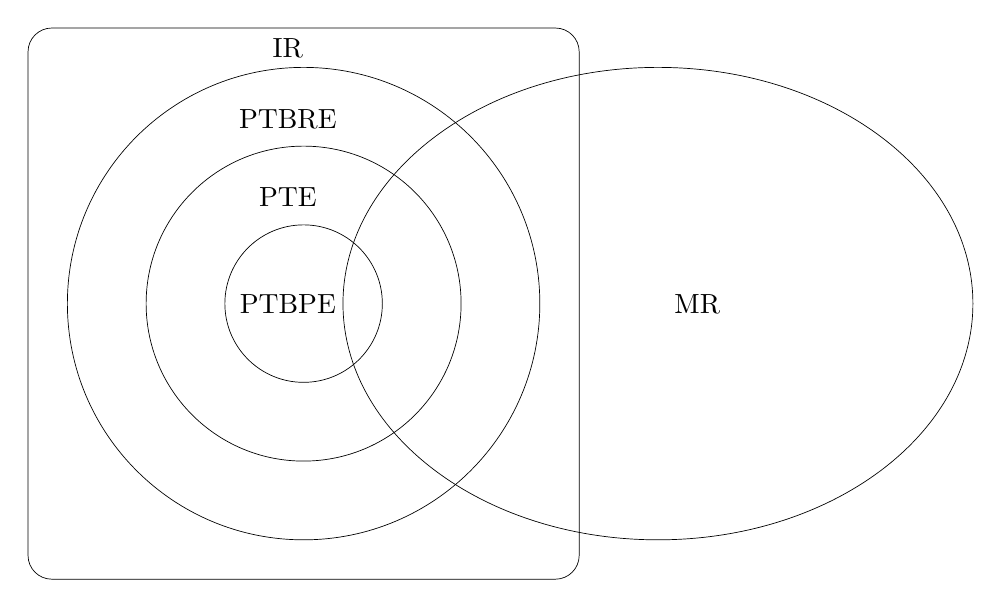
\begin{tikzpicture}[line width=0.25pt]
		\draw (0,0) circle (1);
		\draw (0,0) circle (2);
		\draw (0,0) circle (3);
		\draw[rounded corners=2ex] (-3.5,3.5) rectangle (3.5,-3.5);
		\draw (4.5,0) ellipse (4 and 3);
		\node at (-0.2,0) {PTBPE};
		\node at (-0.2,1.35) {PTE};
		\node at (-0.2,2.35) {PTBRE};
		\node at (-0.2,3.25) {IR};
		\node at (5,0) {MR};
	\end{tikzpicture}
\end{figure}

\section{Symmetric games without ties}

\begin{observation}
	 In a symmetric game $G = (P, S, \uu)$, if a strategy profile $\vecs \in S$ is a PTE, then it lies on the diagonal, i.e., we have $\vecs = (a, a, \dots, a)$ for some strategy $a$.
\end{observation}

\begin{proof}
	If there was a PTE somewhere else than on the diagonal, we would necessarily have multiple PTEs by symmetry, contradicting the uniqueness of PTE.
\end{proof}

\begin{corollary}
	If a symmetric game $G = (P, S, \uu)$ has a PTE $\vecs \in S$ and $\vecs$ is the perfectly transparent $i$-best profile for some player $i \in P$, then $\vecs$ is a PTBPE. 
\end{corollary}

\begin{proof}
	Since $\vecs$ is on the diagonal and it is the perfectly transparent $i$-best profile for some $i \in P$, by symmetry, it must actually be the perfectly transparent $j$-best profile for all $j \in P$, which is the definition of PTBPE.
\end{proof}

\begin{conjecture}
	PTE = PTBPE.
\end{conjecture}

\begin{lemma}
	In a symmetric game $G = (P, S, \uu)$, if a strategy profile $\vecs \in S$ is a PTE, then it is minimax rationalizable.
	Thus, we have PTE\textsuperscript{sym} $\subset$ MR.
\end{lemma}

\begin{proof}
	Suppose for the sake of deriving a contradiction that there is a game $G = (P, S, \uu)$ and a strategy profile $\vecs \in S$ that is a PTE but not minimax rationalizable.
	By definition, this means that there is some player $i \in P$ such that $(s_i, \vecs_{-i}')$ is not minimax rationalizable for any $\vecs' \in S$.
	By symmetry, if this statement holds for one player, then it must hold for all players.
	Let $s_j$ be the strategy that minimax-dominates $s_i$ (i.e. causes that $s_i$ is not minimax rationalizable).
	We denote $\vecs^* = (s_j, s_j, \dots, s_j)$.
	In the round where strategy $s_i$ is eliminated, strategy profile $\vecs^*$ must survive---otherwise strategy $s_j$ would be eliminated as well, but we supposed that $s_j$ is the strategy that caused the elimination of $s_i$.
	Moreover, we must have $u_i(\vecs^*) > u_i(\vecs)\ \forall i \in P$ because $s_j$ minimax-dominates $s_i$.
	This means $\vecs$ is not Pareto-optimal which contradicts $\vecs$ being a PTE.
\end{proof}
